\documentclass{scrartcl} % scrartcl of scrreprt
% Include all project wide packages here.
\usepackage{fullpage}
\usepackage{polyglossia}
\setmainlanguage{dutch}
\usepackage{csquotes}
\usepackage{graphicx}
\usepackage{epstopdf}
\usepackage{pdfpages}
\usepackage{caption}
\usepackage[list=true]{subcaption}
\usepackage{float}
%\usepackage{mathtools}
\usepackage{standalone}
\usepackage{import}
\usepackage{tocloft}
\usepackage{wrapfig}
\usepackage{authblk}
\usepackage{array}
\usepackage{booktabs}
\usepackage[toc,page,title,titletoc]{appendix}
\usepackage{xunicode}
\usepackage{amsmath}
\usepackage{fontspec}
\usepackage{unicode-math}
\usepackage[
    backend=bibtexu,
	texencoding=utf8,
bibencoding=utf8,
    style=ieee,
    sortlocale=nl_NL,
    language=auto
]{biblatex}
\usepackage{listings}
\newcommand{\includecode}[3][c]{\lstinputlisting[caption=#2, escapechar=, style=#1]{#3}}
\newcommand{\superscript}[1]{\ensuremath{^{\textrm{#1}}}}
\newcommand{\subscript}[1]{\ensuremath{_{\textrm{#1}}}}


\newcommand{\chapternumber}{\thechapter}
\renewcommand{\appendixname}{Bijlage}
\renewcommand{\appendixtocname}{Bijlagen}
\renewcommand{\appendixpagename}{Bijlagen}

\usepackage[hidelinks]{hyperref} %<--------ALTIJD ALS LAATSTE

\renewcommand{\familydefault}{\sfdefault}

\setmainfont[Ligatures=TeX]{Myriad Pro}
\setmathfont{Asana Math}
\setmonofont{Lucida Console}

\usepackage{titlesec, blindtext, color}
\definecolor{gray75}{gray}{0.75}
\newcommand{\hsp}{\hspace{20pt}}
\titleformat{\chapter}[hang]{\Huge\bfseries}{\chapternumber\hsp\textcolor{gray75}{|}\hsp}{0pt}{\Huge\bfseries}
\renewcommand{\familydefault}{\sfdefault}
\renewcommand{\arraystretch}{1.2}
\setlength\parindent{0pt}

%For code listings
\definecolor{black}{rgb}{0,0,0}
\definecolor{browntags}{rgb}{0.65,0.1,0.1}
\definecolor{bluestrings}{rgb}{0,0,1}
\definecolor{graycomments}{rgb}{0.4,0.4,0.4}
\definecolor{redkeywords}{rgb}{1,0,0}
\definecolor{bluekeywords}{rgb}{0.13,0.13,0.8}
\definecolor{greencomments}{rgb}{0,0.5,0}
\definecolor{redstrings}{rgb}{0.9,0,0}
\definecolor{purpleidentifiers}{rgb}{0.01,0,0.01}


\lstdefinestyle{csharp}{
language=[Sharp]C,
showspaces=false,
showtabs=false,
breaklines=true,
showstringspaces=false,
breakatwhitespace=true,
escapeinside={(*@}{@*)},
columns=fullflexible,
commentstyle=\color{greencomments},
keywordstyle=\color{bluekeywords}\bfseries,
stringstyle=\color{redstrings},
identifierstyle=\color{purpleidentifiers},
basicstyle=\ttfamily\small}

\lstdefinestyle{c}{
language=C,
showspaces=false,
showtabs=false,
breaklines=true,
showstringspaces=false,
breakatwhitespace=true,
escapeinside={(*@}{@*)},
columns=fullflexible,
commentstyle=\color{greencomments},
keywordstyle=\color{bluekeywords}\bfseries,
stringstyle=\color{bluestrings},
identifierstyle=\color{purpleidentifiers}
}

\lstdefinestyle{vhdl}{
language=VHDL,
showspaces=false,
showtabs=false,
breaklines=true,
showstringspaces=false,
breakatwhitespace=true,
escapeinside={(*@}{@*)},
columns=fullflexible,
commentstyle=\color{greencomments},
keywordstyle=\color{bluekeywords}\bfseries,
stringstyle=\color{redstrings},
identifierstyle=\color{purpleidentifiers}
}

\lstdefinestyle{xaml}{
language=XML,
showspaces=false,
showtabs=false,
breaklines=true,
showstringspaces=false,
breakatwhitespace=true,
escapeinside={(*@}{@*)},
columns=fullflexible,
commentstyle=\color{greencomments},
keywordstyle=\color{redkeywords},
stringstyle=\color{bluestrings},
tagstyle=\color{browntags},
morestring=[b]",
  morecomment=[s]{<?}{?>},
  morekeywords={xmlns,version,typex:AsyncRecords,x:Arguments,x:Boolean,x:Byte,x:Char,x:Class,x:ClassAttributes,x:ClassModifier,x:Code,x:ConnectionId,x:Decimal,x:Double,x:FactoryMethod,x:FieldModifier,x:Int16,x:Int32,x:Int64,x:Key,x:Members,x:Name,x:Object,x:Property,x:Shared,x:Single,x:String,x:Subclass,x:SynchronousMode,x:TimeSpan,x:TypeArguments,x:Uid,x:Uri,x:XData,Grid.Column,Grid.ColumnSpan,Click,ClipToBounds,Content,DropDownOpened,FontSize,Foreground,Header,Height,HorizontalAlignment,HorizontalContentAlignment,IsCancel,IsDefault,IsEnabled,IsSelected,Margin,MinHeight,MinWidth,Padding,SnapsToDevicePixels,Target,TextWrapping,Title,VerticalAlignment,VerticalContentAlignment,Width,WindowStartupLocation,Binding,Mode,OneWay,xmlns:x}
}

%defaults
\lstset{
basicstyle=\ttfamily\small,
extendedchars=false,
numbers=left,
numberstyle=\ttfamily\tiny,
stepnumber=1,
tabsize=4,
numbersep=5pt
}
\addbibresource{../../library/bibliography.bib}

\author{Robin Hes}
\title{EPO3: Eindrapport - Draw-line}

\begin{document}
\section{Draw-line}
\label{sec:draw-line}

%Specs
\subsection{Specificaties}
Draw\_line is gespecificeerd als een module die, wanneer hij ingeschakeld is (en = `1'), en toegang heeft tot het RAM (draw\_can\_access = `1') een lijn van de gewenste kleur (color), van (x0 en y0) en naar (x1 en y1) de gewenste coördinaten naar het VRAM schrijft. Hij doet dit in het niet-actieve screenbuffer (not asb), zodat de lijn na de volgende schermbuffwisseling door de VGA-controller op het scherm getekend wordt. De aansluitingen van de module zijn te vinden in figuur \ref{fig:draw-line-schema}.
%Bij het schrijven van een pixel naar het VRAM dient het adres te bestaan uit het screen buffer waar naar geschreven moet worden (a), de y-coördinaat van de pixel (b) en de x-coördinaat van de pixel (b). Dit levert de volgende adresvorm op: (ayyyyyyyxxxxxxxx)

\begin{figure}[H]
	\centering
	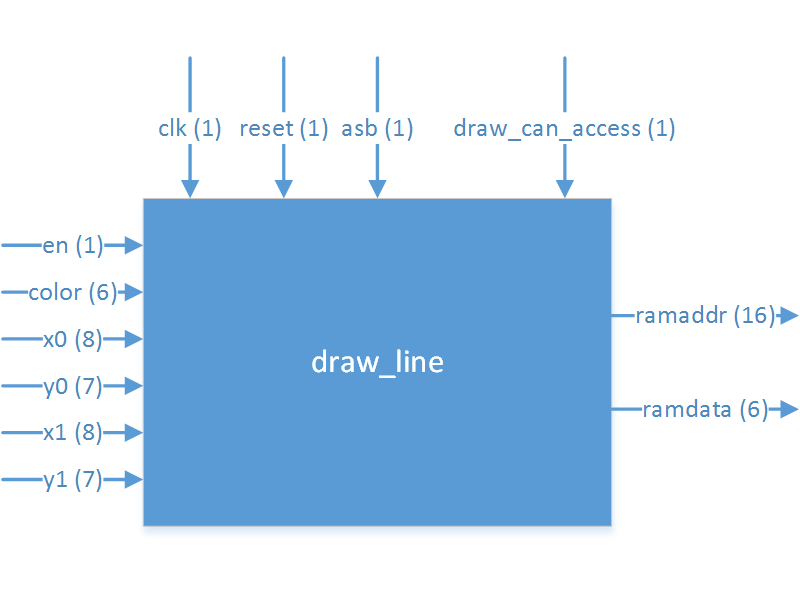
\includegraphics[width=0.75\textwidth]{resource/draw_line.png}
	\caption{Een blokschema van draw\_line, met de namen van de gebruikte in- en uitgangen en tussen haakjes het aantal bits}
	\label{fig:draw-line-schema}
\end{figure}

%Ontwerp en implementatie
\subsection{Ontwerp en implementatie}
Voor dit doeleinde wordt gebruik gemaakt van het lijnalgoritme van Bresenham. Specifiek een voor hardware geöptimaliseerde en gesimplificeerde versie van dat algoritme. \cite{line-alg} Dit algoritme tekent in een loop een rij pixels van een punt naar een ander punt, waarvan de coördinaten per iteratie in de x-richting, y-richting, of beide richtingen verschuiven. De coördinaten van de nieuwe pixel worden berekend aan de hand van het verschil tussen de begin- en eindcoördinaat (dx en dy) en de laatst getekende pixel.
\\\\
De implementatie van de module is een letterlijke implementatie van het eerdergenoemde algoritme. De pseudocode voor dit algoritme is voor de volledigheid opgenomen in bijlage \ref{appsec:pseudocode-bresenham-line}. Het enige probleem bij het omzetten van deze pseudocode naar een VHDL-beschrijving was het feit dat er geen loop gebruikt kan worden om te itereren, omdat er niet meerdere keren naar het VRAM geschreven kan worden per klokslag.
\\
In plaats daarvan is gekozen om in het combinatorische process van de module één iteratie te verwerken (en dus één pixel naar het screen buffer te schrijven). Ook worden in een iteratie de relevante signals (cx, cy en err) zo aangepast dat de volgende executie van het process de volgende pixel tekent en zo verder, totdat het eindpunt bereikt is.
\\
De module begint op x0 en y0 en schuift iedere process-executie op naar een nieuwe pixel, de locatie van deze pixel wordt intern bijgehouden met de signalen cx en cy. De nieuwe pixel kan verschoven zijn in de x- of y-richting of beide richtingen. Dit is afhankelijk van de ``fout'' (het signaal err), die in Bresenham's algoritme berekend wordt, deze fout is afhankelijk van het verschil tussen het start- en eindpunt van de lijn: dx en dy. Naast het verplaatsen van de huidige pixel wordt deze ook bij iedere iteratie weggeschreven naar het VRAM. Dit betekent dat er een kleur in het niet-actieve gedeelte van het VRAM wordt geschreven op het juiste adres. Dit adres (ramaddr) is dan een combinatie van not asb, cy en cx, waar de te schrijven data (ramdata) simpelweg bestaat uit de gegeven kleur (color).

%VHDL simulatie
\subsection{VHDL simulatie}
Voor de eerste simulatie van de VHDL is gebruik gemaakt van ModelSim. In de gebruikte testbench werd de draw\_line module geactiveerd om van- en naar de ingegeven coördinaten een lijn te tekenen in het VRAM. In de waveform van deze testbench was inderdaad te zien dat cx en cy van het startpunt opschoven naar het eindpunt. Ondertussen werden deze coördinaten correct weggeschreven naar het VRAM. Wanneer cx en cy het ingegeven eindpunt hadden bereikt, detecteerde de module bovendien dat hij klaar was en ging het done-signaal netjes omhoog.
\\
In figuur \ref{fig:draw-line-modelsim} is een fragment uit de waveform van deze testbench in ModelSim te zien. De lijn moet in deze testbench getekend worden van punt (10, 87), naar punt (170, 15). In dit fragment is te zien hoe de waarden van cx en cy het eindpunt benaderen totdat dit eindpunt is bereikt. Op dat moment gaat het signaal done omhoog om aan te geven dat de lijn klaar is. Ook is het effect van Bresenham's algoritme zichtbaar. cy benadert zijn doel langzamer dan cx (waar cx elke klokslag wordt opgehoogd, daalt cy juist een keer per twee klokslagen), omdat dx groter is dan dy. Daarnaast zien we dat ramaddr correct is opgebouwd uit not asb, cy en cx, en dat ramdata inderdaad gelijk is aan color.

\begin{figure}[H]
	\centering
	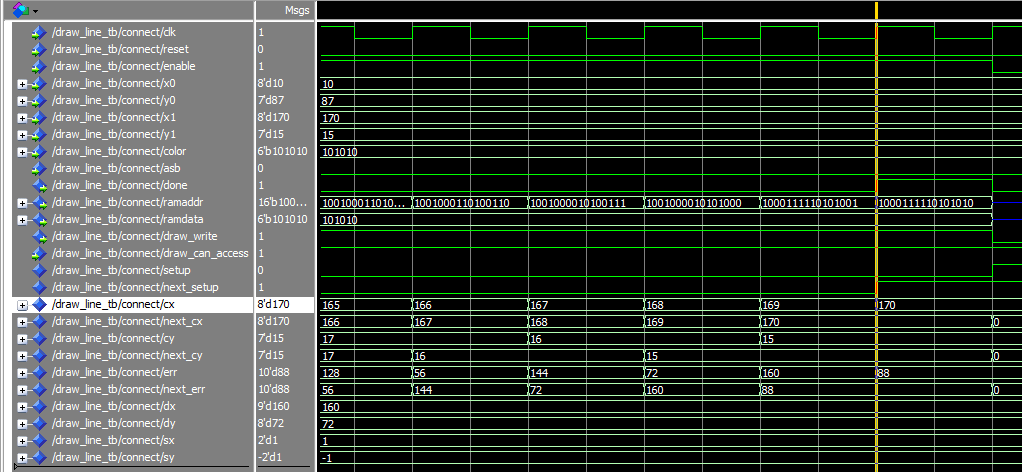
\includegraphics[width=\textwidth]{resource/modelsim.png}
	\caption{Een fragment uit de waveform van de draw-line testbench }
	\label{fig:draw-line-modelsim}
\end{figure}

Ook een test van de gehele GPU, om de inhoud van het VRAM te verifiëren door middel van de SRAMDebugTool, leverde inderdaad een lijn op als resultaat: zie figuur \ref{fig:draw-line-sram-dump}.

\begin{figure}[H]
	\centering
	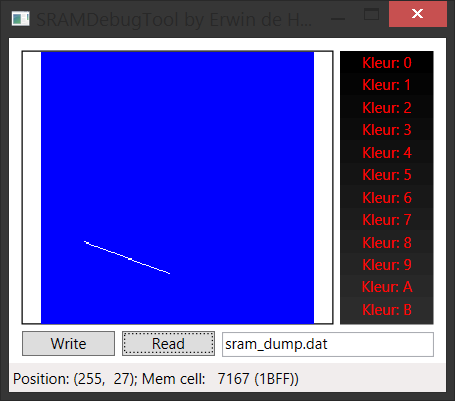
\includegraphics[width=0.6\textwidth]{resource/sram_dump.png}
	\caption{Het VRAM na een GPU testbench, waarin een lijn wordt getekend. De lijn is zichtbaar in het onderste screen buffer}
	\label{fig:draw-line-sram-dump}
\end{figure}

%Synthese
\subsection{Synthese en lay-out}
De draw-line module verwerkt relatief grote vectors. Hij moet deze opslaan en er moeten optel- en shiftoperaties op uitgevoerd worden. Dit alles resulteert in een synthese die een vrij groot transistoroppervlak oplevert. De synthesizer levert een ``total cell area'' op van 3190. Madonna levert bij dit soort aantallen transistoren niet zulke goede resultaten, dus het plaatsen van de rijen is handmatig gedaan. Het blijkt dat het beste resultaat behaald wordt met het plaatsen van 18 rijen, waar de onderlinge afstand tussen de cellen 6 bedraagt. Ook is de optie ``vary distance'' uitgeschakeld. Wanneer vervolgens Trout wordt losgelaten op deze plaatsing, levert dit een aantal van 23706 transistoren op, waarvan er 6393 daadwerkelijk gebruikt zijn. De efficiëntie voor deze module bedraagt dan 26.97\%.

%Switchlevel test
\subsection{Switch-level simulatie}
De gesynthetiseerde schakeling is gesimuleerd met SLS met de originele testbench en vervolgens vergeleken met de resultaten van die testbench. Dit vergelijk leverde de verwachte resultaten op, dus gesteld mag worden dat de synthese goed is verlopen. Na het maken van een lay-out is wederom gesimuleerd met SLS en vergeleken met de originele testbench. Ook dit leverde het gewenste resultaat, dus ook de hardware-implementatie van draw\_line is geslaagd.

%Conclusie
\subsection{Conclusie}
Iedere simulatie van draw\_line leverde het gewenste resultaat op, dus ook een SoG-implementatie van de module in de uiteindelijke chip, zou in theorie moeten functioneren. Toch is als minpunt ook aan te wijzen dat de module behoorlijk uit de kluiten gewassen is. Met een oppervlak van bijna 24000 transistoren is het de grootste module op de chip en neemt hij ruim een vierde van het oppervlak in. Door de verschillende operaties die in draw\_line worden uitgevoerd los te koppelen en als component te gebruiken zou de efficiëntie van de module verhoogd kunnen worden. Ook zouden andere modules dan eventueel gebruik kunnen maken van deze optellers en registers.

\end{document}
